\newpage
\section{Theoretical Analysis}
\label{sec:analysis}

In this section we will present the answers to questions~\ref{sec:exercise1} to~\ref{sec:exercise6}. For solving purposes, all the unkown currents used in the node analysis were considered to be diverging from the node. The node $V_4$ is connected to the ground (GND) in every exercise, the voltage in it being 0V.

\subsection{Exercise 1}
\label{sec:exercise1}


%---------------Theoretical Analysis Exercise 1--------------------------------------------------------%
 
The first thing which must be noticed is that there is an independent voltage source ($V_s$) and a linear current controlled voltage source ($V_d$) in this circuit. Knowing that a nodal analysis can't include the analysis of nodes that are connected to voltage sources, it becomes clear that is useless to analyze nodes 1 and 4 (connected to $V_s$) and also nodes 5 and 8 (connected to $V_d$) using this method.

From figure~\ref{fig:??}, we can easily conclude that there are 11 unknown variables: $V_b$, $I_b$, $V_d$, $I_d$, $V_1$, $V_2$, $V_3$, $V_5$, $V_6$, $V_7$ and $V_8$. In this exercise, $V_s$ is constant and the capacitor is assumed to be also constant and fully charged, meaning that the current $I_c$ is 0 (open circuit behavior).

For the node analysis, it is necessary to consider 7 linearly independent equations to reach all the values corresponding to the voltages in each node and consequently solve the circuit. As referred above, it is possible to use the nodal method to analyze nodes 2, 3, 6 and 7.

We begin by establishing the following equations, being that equations ~\ref{eq:given11} and ~\ref{eq:given12} were given by the professor. Equation ~\ref{eq:vb1} was obtained by relating the voltage difference between nodes 2 and 5 to the voltage $V_b$. Finally, by using Ohm's Law for resistor $R_6$ and remembering that $V_4$ is null, we get the last equation (\ref{eq:id1}) for $I_d$.

\begin{equation}
  I_{b} = K_{b}V_{b} ,
  \label{eq:given11}
\end{equation}

\begin{equation}
  V_{d} = K_{d}I_{d} ,
  \label{eq:given12}
\end{equation}

\begin{equation}
  V_{b} = V_{2} - V_{5} ,
  \label{eq:vb1}
\end{equation}

\begin{equation}
  I_{d} = -V_{7}G_{6} ,
  \label{eq:id1}
\end{equation}

The equation written below (\ref{eq:node11}) is a direct consequence of our choice of connecting node 4 to the ground (GND), because this choice makes evident that the value of $V_4$ is 0 and then:
\begin{equation}
  V_{1} - V_{s} = 0,
  \label{eq:node11}
\end{equation}

By analysing node 2 using Kirchoff's Current Law and Ohm's Law for the resistors $R_1$, $R_2$ and $R_3$, we get the following equation:

\begin{equation}
  (V_{3} - V_{1})G_{1} + (V_{2} - V_{3})G_{2} + (V_{2} - V_{5})G_{3}= 0,
  \label{eq:node12}
\end{equation}

The following equation (\ref{eq:node13}), in which was also used Kirchoff's Current Law and Ohm's Law for resistor $R_2$, refers to node 3. Here we consider the given equation ~\ref{eq:given11} and the equation ~\ref{eq:vb1} to substitute the current $I_b$.

\begin{equation}
  (V_{3} - V_{2})G_{2} - (V_{2} - V_{5})K_{b} = 0,
  \label{eq:node13}
\end{equation}

For node 6, the ensuing equation (\ref{eq:node16}) was figured out by resorting to Ohm's Law for the resistor $R_5$ and Kirchoff's Current Law. Equations ~\ref{eq:given11} and~\ref{eq:vb1} were once again used to avoid using $I_b$. Remember that, for this exercise, $I_c$ is null.

\begin{equation}
  (V_{6} - V_{5})G_{5} + (V_{2} - V_{5})K_{b} = 0,
  \label{eq:node16}
\end{equation}

Finally, for node 7, Kirchoff's Circuit Law and Ohm's Law (for resistors $R_6$ and $R_7$) were used to establish the following mathematical relation:

\begin{equation}
  V_{7}G_{6} + (V_{7} - V_{8})G_{7} = 0,
  \label{eq:node17}
\end{equation}

Since there are 7 unkown varibles, we need two more equations. The first one (\ref{eq:vd1}) is obtained by relating $V_d$ to the voltage difference in nodes 5 and 8 and replacing $V_d$ for the equations~\ref{eq:given12} and~\ref{eq:id1}.

\begin{equation}
  -V_{7}G_{6}K_{d} - (V_{5} - V_{8}) = 0,
  \label{eq:vd1}
\end{equation}

Ultimately, to discover the last equation, there are some theoretical concepts that must be considered. Kirchoff's Current Law implies that there is no current stuck at any node. It is also known that neither voltage sources nor resistors retain current. Then, any branch that only contains one of the said elements does not retain current as well. Merging the two branches placed on the left side of circuit (branch containing $V_s$ with branch containing $R_6$) and calling Supernode to the result of this merger, it is still true that no current is retained in the Supernode. Then, considering that all unkown currents are diverging from the nodes, the resultant equation (\ref{eq:supernode1}) is the one written right below.

\begin{equation}
  (V_{1} - V_{2})G_{1} - V_{5}G_{7} - V_{7}G_{6} = 0,
  \label{eq:supernode1}
\end{equation}

A system with the 7 linearly independent equations and 7 variables (regarding the voltage in each node) is, of course, possible to solve but not easy (and certainly not pratical) to deal with. The following matrix equation (\ref{eq:nodalmatrix1}) summarizes the 7 referred equations so it is easier to read and to instantaneously solve (by using Octave).
\begin{equation}
\left[ \begin{array}{ccccccc} 
		1 & 0 & 0 & 0 & 0 & 0 & 0 \\ 
		-G_1 & G_1+G_2+G_3 & -G_2 & -G_3 & 0 & 0 & 0 \\
		0 & -G_2-K_b & G_2 & K_b & 0 & 0 & 0 \\ 
		0 & K_b & 0 & -K_b-G_5 & G_5 & 0 & 0  \\ 
		0 & 0 & 0 & 0 & 0 & G_6+G_7 & -G_7  \\ 
		G_1 & -G_1 & 0 & -G_4 & 0 & -G_6 & 0  \\ 
		0 & 0 & 0 & -1 & 0 & -K_dG_6 & 1 \\ 

\end{array} \right]
\times \left[ \begin{array}{c} V_1 \\ V_2 \\ V_3 \\  V_5 \\ V_6 \\ V_7 \\ V_8 \end{array} \right] =
\left[ \begin{array}{c} V_s \\ 0 \\ 0 \\ 0 \\ 0 \\ 0 \\ 0  \end{array} \right]
\label{eq:nodalmatrix1}
\end{equation}

\label{sec:Exercise 1}
\begin{figure}[!ht] \centering
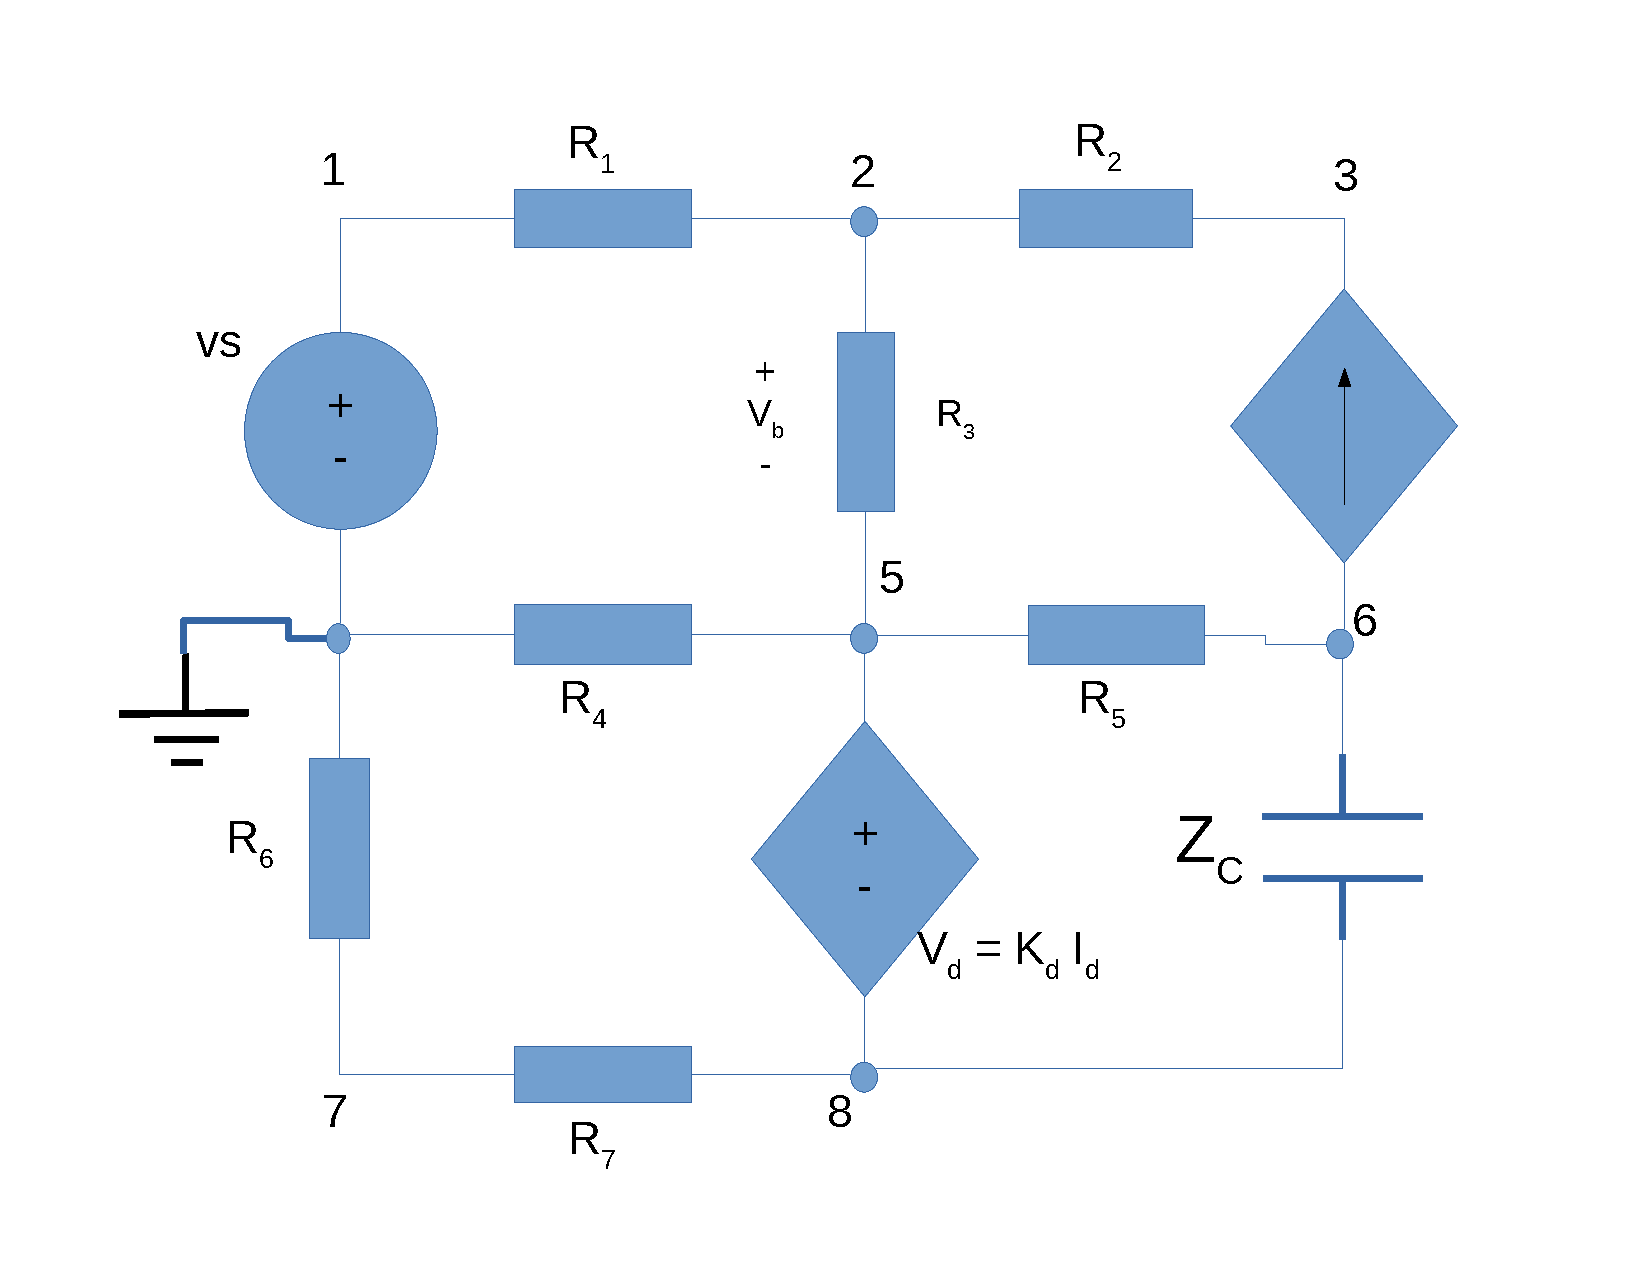
\includegraphics[width=0.8\linewidth]{circuit_node.pdf}
\caption{Representation of the current directions considered.}
\label{fig:nodeanalysis1}
\end{figure}

To find all the required branches' currents we can use Ohm's Law for each resistor, which can be seen in equations~\ref{eq:ohm11} to~\ref{eq:ohm17}: Now we no longer consider the currents to be diverging from the nodes, but assume the directions shown in figure~\ref{fig:nodeanalysis1}.


\begin{equation}
  R_1[i] = \frac{V_1 - V_2}{R_1},
  \label{eq:ohm11}
\end{equation}

\begin{equation}
  R_2[i] = \frac{V_2 - V_3}{R_2},
  \label{eq:ohm12}
\end{equation}

\begin{equation}
  R_3[i] = \frac{V_5 - V_2}{R_3},
  \label{eq:ohm13}
\end{equation}

\begin{equation}
  R_4[i] = \frac{V_5}{R_4},
  \label{eq:ohm14}
\end{equation}

\begin{equation}
  R_5[i] = \frac{V_6 - V_5}{R_5},
  \label{eq:ohm15}
\end{equation}

\begin{equation}
  R_6[i] = -\frac{V_7}{R_6},
  \label{eq:ohm16}
\end{equation}

\begin{equation}
  R_7[i] = \frac{V_7 - V_8}{R_7},
  \label{eq:ohm17}
\end{equation}

Here we have tables~\ref{table:theoretical_1} and~\ref{table:??} in which the final values of the unkown variables are printed. 

\begin{table}[!ht]
\centering
\begin{tabular}{ |c|c|} 
 \hline
 {\bf Node} & {\bf Voltage[V]} \\ 
 \hline\hline
  $V_b$ & \partialinput{1}{1}{theoretical_1.tex}\\ 
 \hline
  $V_d$ & \partialinput{2}{2}{theoretical_1.tex} \\ 
 \hline
 $V_1$ & \partialinput{3}{3}{theoretical_1.tex} \\ 
 \hline
 $V_2$ & \partialinput{4}{4}{theoretical_1.tex} \\ 
 \hline
 $V_3$ & \partialinput{5}{5}{theoretical_1.tex} \\ 
 \hline
 $V_5$ & \partialinput{6}{6}{theoretical_1.tex} \\ 
 \hline
 $V_6$ & \partialinput{7}{7}{theoretical_1.tex} \\ 
\hline
 $V_6$ & \partialinput{8}{8}{theoretical_1.tex} \\ 
 \hline
 $V_8$ & \partialinput{9}{9}{theoretical_1.tex} \\
 \hline
\end{tabular}
\caption{Voltage and Current values(Exercise 1)}
\begin{tabular}{ |c|c|} 
 \hline
 {\bf Branch} & {\bf Current[A]}\\ 
 \hline\hline
 $I_b$ & \partialinput{10}{10}{theoretical_1.tex} \\ 
 \hline
 $I_c$ & \partialinput{11}{11}{theoretical_1.tex} \\
 \hline
 $R_6 = I_d$ & \partialinput{12}{12}{theoretical_1.tex} \\
 \hline
 $R_1$ & \partialinput{13}{13}{theoretical_1.tex} \\ 
 \hline
  $R_2$ & \partialinput{14}{14}{theoretical_1.tex} \\ 
 \hline
  $R_3$ & \partialinput{15}{15}{theoretical_1.tex} \\  
 \hline
 $R_4$ & \partialinput{16}{16}{theoretical_1.tex} \\ 
 \hline
 $R_5$ & \partialinput{17}{17}{theoretical_1.tex} \\  
 \hline
  $R_7$ & \partialinput{19}{19}{theoretical_1.tex} \\  
 \hline
\end{tabular}
\label{table:theoretical_1}
\end{table}

%\begin{figure}[!ht] \centering
%\caption{Final solution of $v_6(t)$ and $v_s(t)$ in the interval $[-5,20]ms$}
%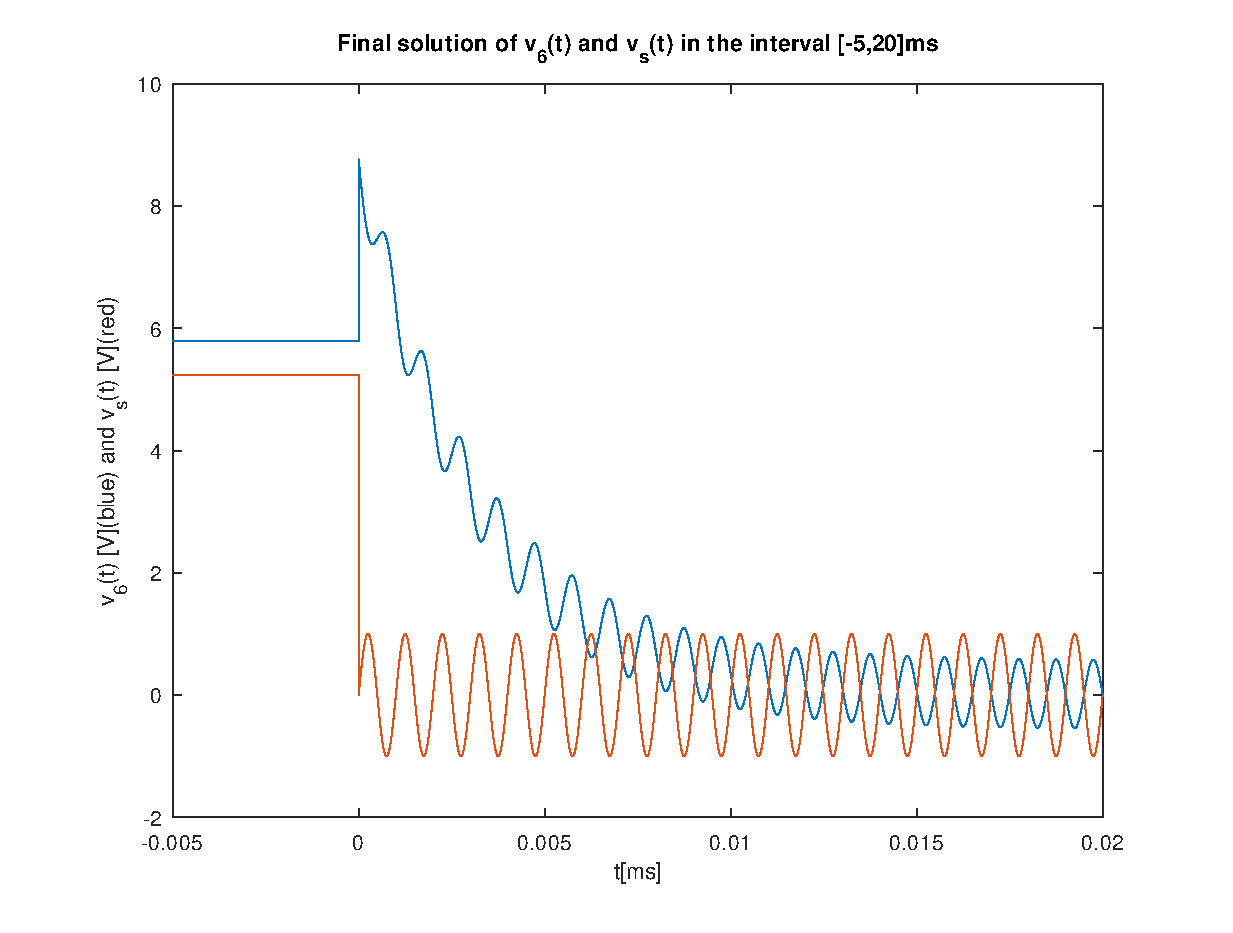
\includegraphics[width=0.8\linewidth]{theoretical_5.eps}
%\label{fig:circuit}
%\end{figure}


\subsection{Exercise 2}
\label{sec:exercise2}


%---------------Theoretical Analysis Exercise 2--------------------------------------------------------%

\label{sec:Exercise 2}
\begin{figure}[!ht] \centering
\includegraphics[width=0.8\linewidth]{circuit_v_x.pdf}
\caption{Circuit representation for exercise 2.}
\label{fig:nodeanalysis2}
\end{figure}

To solve this exercise, we first needed to get the value of $V_x$, which we did by applying the equation given by the professor (\ref{eq:vx2}), using the values of $V_6$ and $V_8$ we got from the matrix~\ref{eq:nodalmatrix1}. This value corresponds to the voltage in the capacitor that now functions as a voltage source, as seen in figure~\ref{fig:nodeanalysis2}. This happens because, as mentioned before, we can assume that an infinite time as passed until t=0 and it is fully charged, meaning it starts with the voltage given before we start the time.

To get the value intended of $R_eq$, it is necessary to achieve the value of the current supplied by the new voltage source $V_x$, $I_x$. This is done by the following node analysis.

Since $V_s$ is now null, it can be ignored, making it so that node 1 is the same as node 4, with a voltage of 0V. This means that the node 4 that could not be used for node analysis before provides another equation. However, the voltage source $V_x$ is connected to node 6, this one being no longer useful. For this exercise, we have 6 unkown variables for the node voltages ($V_2$, $V_3$, $V_5$, $V_6$, $V_7$ and $V_8$) and we can analyse the nodes 2, 3, 4 and 7.

These 3 equations are all obtained from the exercise above (reference to equations~\ref{eq:node12},~\ref{eq:node13} and~\ref{eq:node17}) to, but assuming that $V_1$ is null, since in the nodes 2, 3 and 7, nothing has changed from the previous circuit, when it comes to connected components.

\begin{equation}
  (V_{3} - V_{1})G_{1} + (V_{2} - V_{3})G_{2} + (V_{2} - V_{5})G_{3}= 0,
  \label{eq:node22}
\end{equation}

\begin{equation}
  (V_{3} - V_{2})G_{2} - (V_{2} - V_{5})K_{b} = 0,
  \label{eq:node23}
\end{equation}

\begin{equation}
  V_{7}G_{6} + (V_{7} - V_{8})G_{7} = 0,
  \label{eq:node27}
\end{equation}

From node 1, we can achieve the equation below by using Kirchoff's Circuit Law and Ohm's Law for resistors $R_1$, $R_6$ and $R_7$.

\begin{equation}
  -V_{7}G_{6} - V_{5}G_{4} - V_{2}G_{1} = 0,
  \label{eq:node21}
\end{equation}


The following equations are also trivial. The first one, equation~\ref{eq:vd2} is explained in the first exercise (reference to equation~\ref{eq:vd1}) and equation ~\ref{eq:given2} is given by the professor and can be used as the value of $V_x$ is constant.

\begin{equation}
  -V_{7}G_{6}K_{d} - (V_{5} - V_{8}) = 0,
  \label{eq:vd2}
\end{equation}


\begin{equation}
  V_{6} - V_{8} = V_{x},
  \label{eq:given2}
\end{equation}

These equations are now enough to solve for the value of $V_2$, $V_3$, $V_5$, $V_6$, $V_7$ and $V_8$, using the matrix below. This was solve in Octave as it was not pratical to solve it normally and the results are presented in table~\ref{table:??}.

\begin{equation}
\left[ \begin{array}{cccccc} 
		G_1+G_2+G_3 & -G_2 & -G_3 & 0 & 0 & 0 \\
		-G_2-K_b & G_2 & K_b & 0 & 0 & 0 \\ 
		0 & 0 & 0 & 0 & G_6+G_7 & -G_7  \\ 
		-G_1 & 0 & -G_4 & 0 & -G_6 & 0  \\ 
		0 & 0 & -1 & 0 & -K_dG_6 & 1 \\ 
		0 & 0 & 0 & 1 & 0 & -1 \\ 
\end{array} \right]
\times \left[ \begin{array}{c} V_2 \\ V_3 \\  V_5 \\ V_6 \\ V_7 \\ V_8 \end{array} \right] =
\left[ \begin{array}{c} 0 \\ 0 \\ 0 \\ 0 \\ 0 \\ V_x  \end{array} \right]
\label{eq:nodalmatrix2}
\end{equation}

The value of $I_x$ is achieved by using Kirchhoff Current Law (KCL) in node 6. We considered the currents to be diverging from the node. From this, the equation below was obtained.

\begin{equation}
  I_{x} + (V_{2} - V_{5})K_{b} + (V_{5} - V_{6})G_{6} = 0,
  \label{eq:ix2}
\end{equation}

Finally, we get the value of $R_eq$:

\begin{equation}
  R_eq = \frac{V_x}{I_x},
  \label{eq:ohm14}
\end{equation}

The values of $I_x$ and $R_eq$ are then, correspondingly, 0000 mA and 000000 k ??.


\subsection{Exercise 3}
\label{sec:exercise3}


%---------------Theoretical Analysis Exercise 3--------------------------------------------------------%



\subsection{Exercise 4}
\label{sec:exercise4}


%---------------Theoretical Analysis Exercise 4--------------------------------------------------------%

For this exercise, to find the forced solution $V_6f$(t), we will work with the frequency f = 1000 Hz and the phasor voltage source $V_s$. Since the voltage source for t>0 is $v_s$(t) = sen(2$\pi$ft), to simplify the calculations and as suggested, we will work with the absolute of $V_s$, which was given and it is 1V. 

The node analysis for this exercise is pretty similar to the one in \ref{sec:exercise1} as the voltage source is once again $V_s$ and the capacitor no longer works as a voltage source. This means that we now have 7 varibles $V_1$, $V_2$, $V_3$, $V_5$, $V_6$, $V_7$ and $V_8$ and we can use the node method in nodes 2, 3, 6 and 7, since all the other ones are connected to voltage sources.

Equations \ref{node42} to \ref{supernode4} were all obtained from the node analysis in exercise 1. The first three are achieved, correspondingly, by nodes 2,3 and 7. The second to last equation refers to the current controlled voltage source $V_d$. Finally, the last one is the supernode that we got from merging the two branches placed on the left side of circuit.

\begin{equation}
  (V_{3} - V_{1})G_{1} + (V_{2} - V_{3})G_{2} + (V_{2} - V_{5})G_{3}= 0,
  \label{eq:node42}
\end{equation}

\begin{equation}
  (V_{3} - V_{2})G_{2} - (V_{2} - V_{5})K_{b} = 0,
  \label{eq:node43}
\end{equation}


\begin{equation}
  V_{7}G_{6} + (V_{7} - V_{8})G_{7} = 0,
  \label{eq:node47}
\end{equation}


\begin{equation}
  -V_{7}G_{6}K_{d} - (V_{5} - V_{8}) = 0,
  \label{eq:vd4}
\end{equation}

\begin{equation}
  (V_{1} - V_{2})G_{1} - V_{5}G_{7} - V_{7}G_{6} = 0,
  \label{eq:supernode4}
\end{equation}

The seventh and final equation (\ref{eq:node67}) necessary to complete the matrix is obtained by analysing node 6, using Kirchoff's Circuit Law and Ohm's Law for the resistor $R_5$. The equation for $V_b$ was secured previously (\ref{eq:vb1}). Because we are working with phasors, equations \ref{eq:caphasor1} and \ref{eq:caphasor2} are used to figure out the current flowing through the capacitor, by using its impendance $Z_c$.


\begin{equation}
  I_{c}Z_{c} = V_{c},
  \label{eq:caphasor1}
\end{equation}

\begin{equation}
 Y_c = \frac{1}{Z_c},
  \label{eq:caphasor2}
\end{equation}

\begin{equation}
   (V_{6} - V_{5})G_{5} + (V_{2} - V_{5})K_{b} + (V_{6} - V_{8})Y_{c} = 0,
  \label{eq:node67}
\end{equation}

From this we get the following matrix, that was solved in Octave. The results are printed on the table~\ref{table:??}.

\begin{equation}
\left[ \begin{array}{ccccccc} 
		1 & 0 & 0 & 0 & 0 & 0 & 0 \\ 
		-G_1 & G_1+G_2+G_3 & -G_2 & -G_3 & 0 & 0 & 0 \\
		0 & -G_2-K_b & G_2 & K_b & 0 & 0 & 0 \\ 
		0 & K_b & 0 & -K_b-G_5 & G_5+Y_c & 0 & -Y_c  \\ 
		0 & 0 & 0 & 0 & 0 & G_6+G_7 & -G_7  \\ 
		G_1 & -G_1 & 0 & -G_4 & 0 & -G_6 & 0  \\ 
		0 & 0 & 0 & -1 & 0 & -K_dG_6 & 1 \\ 

\end{array} \right]
\times \left[ \begin{array}{c} V_1 \\ V_2 \\ V_3 \\  V_5 \\ V_6 \\ V_7 \\ V_8 \end{array} \right] =
\left[ \begin{array}{c} V_s \\ 0 \\ 0 \\ 0 \\ 0 \\ 0 \\ 0  \end{array} \right]
\label{eq:nodalmatrix4}
\end{equation}








